\begin{figure}[htbp]
    \centering
    \begin{minipage}[t]{0.58\textwidth}
    \centering
    \resizebox{\linewidth}{!}{%
    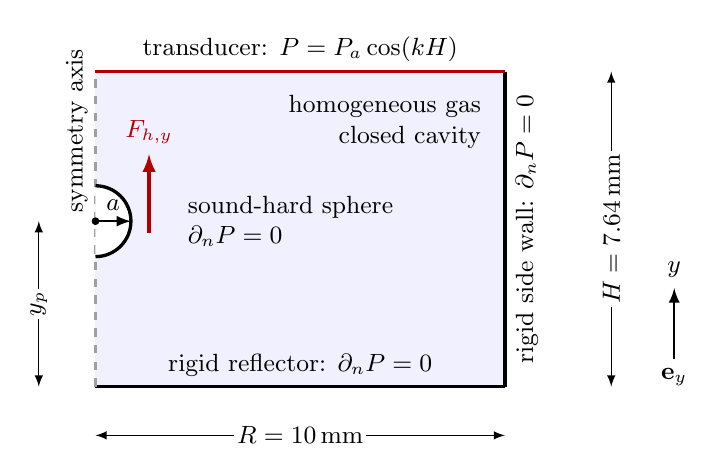
\begin{tikzpicture}[x=1cm,y=1cm,>=latex,font=\small]
        \def\domainR{5.2}
        \def\domainH{4.0}
        \def\particleY{2.1}
        \def\particleR{0.45}

        % Meridional half-domain of the axisymmetric cavity.
        \fill[blue!6] (0,0) rectangle (\domainR,\domainH);
        \draw[very thick] (0,0) -- (\domainR,0);
        \draw[very thick] (\domainR,0) -- (\domainR,\domainH);
        \draw[red!70!black,very thick] (0,\domainH) --
            (\domainR,\domainH);
        \draw[gray!75,dashed,thick] (0,0) -- (0,\domainH);

        % Resolved sphere: a semicircle in the meridional half-domain.
        \fill[white]
            (0,{\particleY+\particleR})
            arc[start angle=90,end angle=-90,radius=\particleR] -- cycle;
        \draw[black,very thick]
            (0,{\particleY+\particleR})
            arc[start angle=90,end angle=-90,radius=\particleR];
        \fill (0,\particleY) circle (1.4pt);
        \draw[->,thick] (0,\particleY) -- (\particleR,\particleY)
            node[midway,above] {$a$};
        \draw[->,red!70!black,very thick]
            (0.68,{\particleY-0.15}) -- (0.68,{\particleY+0.85})
            node[above] {$F_{h,y}$};

        % Geometry dimensions.
        \draw[<->] (-0.72,0) -- (-0.72,\particleY)
            node[midway,fill=white,inner sep=1pt,rotate=90] {$y_p$};
        \draw[<->] (6.55,0) -- (6.55,\domainH)
            node[midway,fill=white,inner sep=1pt,rotate=90]
            {$H=7.64\,\mathrm{mm}$};
        \draw[<->] (0,-0.62) -- (\domainR,-0.62)
            node[midway,fill=white,inner sep=1pt]
            {$R=10\,\mathrm{mm}$};

        % Boundary-condition and domain labels.
        \node[above] at ({0.5*\domainR},\domainH)
            {transducer: $P=P_a\cos(kH)$};
        \node[above] at ({0.5*\domainR},0)
            {rigid reflector: $\partial_nP=0$};
        \node[rotate=90,fill=white,inner sep=1pt] at
            (5.48,{0.5*\domainH})
            {rigid side wall: $\partial_nP=0$};
        \node[rotate=90,fill=white,inner sep=1pt] at (-0.24,3.25)
            {symmetry axis};
        \node[align=left,anchor=west] at (1.05,\particleY)
            {sound-hard sphere\\$\partial_nP=0$};
        \node[anchor=north east,align=right] at
            ({\domainR-0.18},{\domainH-0.18})
            {homogeneous gas\\closed cavity};

        \draw[->,thick] (7.35,0.35) -- (7.35,1.25)
            node[above] {$y$};
        \node at (7.35,0.12) {$\mathbf e_y$};
    \end{tikzpicture}
    }\\[-0.2em]
    \textbf{(a)} Domain and boundary conditions
    \end{minipage}\hfill
    \begin{minipage}[t]{0.38\textwidth}
    \centering
    
\includegraphics[width=\linewidth,trim=300 400 500 400,clip]{mesh_gorkov_local.png}\\[-0.2em]
    \textbf{(b)} Local mesh
    \end{minipage}
    \caption{Rigid-sphere Gorkov case: (a) closed cavity and boundary
    conditions, with the sphere enlarged; (b) illustrative local mesh at
    $h_s/a=0.2$.  Quantitative levels are listed in
    \cref{tab:gorkovMeshConvergence}.  The mesh is a $1^\circ$ axisymmetric
    wedge; no PML is active.}
    \label{fig:gorkovDomainSchematic}
\end{figure}
